\chapter{Data Processing}
\label{ch:data-processing}

In the trivial recommender that we introduced in the introduction, we used a method \lstinline{get_availability} and in the MPIR, we used a method \lstinline{get_item_popularities}. We glossed over the details of these two functions, and hoped the choice of naming would provide sufficient context about what their function was. 

Now we wish to start unpacking the details of some of this complexity, and see what the toolsets are for online and offline collectors.

\section{Hydrating your system}

\subsection{PySpark}

Spark is an extremely general computing library, with APIs for Java, Python, SQL, and Scala. PySpark's role in many ML pipelines is for data processing and transformation of the largest scale datasets in your pipeline. 

Recall that the user-item matrix is the linear-algebraic representation of all of the triples of users, items, and the user's rating of the item. These triples are not naturally occurring in the wild–most commonly, you begin with log files from your system:

\begin{lstlisting}[language=python]
{
	'page_view_id': 'd15220a8e9a8e488162af3120b4396a9ca1', 
	'anonymous_id': 'e455d516-3c08-4b6f-ab12-77f930e2661f', 
	'view_tstamp': 2020-10-29 17:44:41+00:00, 
	'page_url': 'https://bookshop.org/lists/bookshop-org-best-sellers-of-the-week', 
	'page_url_host': 'bookshop.org', 
	'page_url_path': '/lists/bookshop-org-best-sellers-of-the-week', 
	'page_title': 'Best Sellers of the Week', 
	'page_url_query': None, 
	'authenticated_user_id': 15822493.0, 
	'url_report_id': 511629659.0, 
	'is_profile_page': False, 
	'product_viewed': 'list', 
}
\end{lstlisting}

These are the kinds of events that you consume from Engineering, and are likely stored in your columnar database. For data like these, utilizing SQL syntax will be our entry point.

PySpark provides a convenient SQL api, and based on your infrastructure, will allow you to write what looks like SQL queries against a potentially massive dataset:

\begin{lstlisting}[language=Python]
user_item_view_counts_qry = """
SELECT 
  page_views.authenticated_user_id
  , page_views.page_url_path
  , COUNT(DISTINCT page_views.page_view_id) AS count_views 

FROM prod.page_views
JOIN prod.dim_users 
	ON page_views.authenticated_user_id = dim_users.authenticated_user_id 

WHERE DATE page_views.view_tstamp >= '2017-01-01'
	AND dim_users.country_code = 'US'

GROUP BY 
	page_views.authenticated_user_id
  , page_views.page_url_path

ORDER BY 3, page_views.authenticated_user_id
"""

user_item_view_counts_sdf = spark.sql(user_item_view_counts_qry)
\end{lstlisting}

Here is a simply SQL query assuming the log schema above, that would allow you to see for each user-item pair, how many times that user has viewed that pair. The convenience of writing pure SQL here means that we can use our experience in columnar databases to quickly ramp up on Spark. The major advantage of Spark, however, is not yet on display. When executing the above in a Spark Session, this query will not be immediately run. This query will be staged for execution, but Spark waits until you use this data downstream in a way that \emph{requires immediate execution} before it begins doing so. This is called lazy-evaluation, and it allows you to work on your data object without every change and interaction immediately being applied. I'll refer you to more serious treatments of Spark for details, but there's one more important characteristic of the Spark paradigm that is essential to discuss.

Spark is natively a distributed computing language. In particular, this means that the above query, even after I force it to execute, will store its data on multiple computers. Spark works via a \emph{driver program} in your program or notebook, which drives a \emph{cluster manager}, which in turn coordinates \emph{executors} on \emph{worker nodes.} When I query data with Spark, instead of all of that data being returned into a DataFrame in memory on the computer I'm using, parts of that data are sent to memory on the executors. And when I do some transformation on the DataFrame, it is applied appropriately on the pieces of the DataFrame that are stored on each of the executors. If this sounds a bit like magic, that's because it is. Spark is a layer of technology that allows the ML Engineer to program as if they're working on one machine, and have those changes take effect on an entire cluster of machines. 

It's important to caveat that all of this does not come for free; both lazy-evaluation and distributed DataFrames come at a cost of needing additional thought when writing programs. Even though Spark makes a lot of this work far easier, understanding how to write efficient code in this paradigm that works with the architecture but still achieves complicated goals, can require a career's worth of experience. 

Returning to Recommendation Systems, and in particular the offline Collector, we want to use PySpark to build the types of data sets needed to train our models. One simple thing you may wish to do with PySpark is the above: transform your logs data into the appropriate form for training a model. In our simple query above, we applied a few filters to our data, and grouped by user and item to get number of views. There are a variety of other tasks that may fit naturally into this paradigm; perhaps adding user or item features stored in other databases, or high-level aggregations.

In our MPIR, we asked for \lstinline{get_item_popularities}, and we sorta assumed a few things:

\begin{itemize}
\item this would return the count of each item's times being chosen
\item this method would be fast
\end{itemize}

The second point is important if this is going to be called in real time. So how might Spark come into play?

First, let's assume we have a lot of data, enough that I can't get it all to fit into my little MacBook Pro's memory. Additionally, let's continue to use the above schema. We can write an even simpler query:

\begin{lstlisting}[language=Python]
item_popularity_qry = """
SELECT 
  page_views.page_url_path
  , COUNT(DISTINCT page_views.authenticated_user_id) AS count_viewers 

FROM prod.page_views
JOIN prod.dim_users 
	ON page_views.authenticated_user_id = dim_users.authenticated_user_id 

WHERE DATE page_views.view_tstamp >= '2017-01-01'
	AND dim_users.country_code = 'US'

GROUP BY 
	page_views.page_url_path

ORDER BY 2
"""

item_view_counts_sdf = spark.sql(item_popularity_qry)
\end{lstlisting}

We can now write this aggregated list of \lstinline{(item, count)} pairs to an app database to serve \lstinline{get_item_popularities}, something that doesn't require us to do any parsing when this is called, or potentially we can take some subset of the top-$N$ of this list and store it in memory. Either way, we've separated concerns of parsing all of our log data, and doing aggregation, from the \lstinline{get_item_popularities} function call in real-time. 

This example used an overly-simple data aggregation, one just as easy to do in something like PostgreSQL, so why bother? The first reason is scalability. Spark is really built to scale horizontally, which means that as the data we need to access grows, we merely add more and more worker nodes. The second reason is that PySpark is more than just SparkSql; anyone who's  done complicated SQL queries can probably agree that the power and flexibility of SQL is enormous, but frequently certain tasks you want to achieve require a lot of creativity to carry out in the fully SQL environment. PySpark gives you all the expressiveness of Pandas DataFrames, Python functions and classes, and a simple interface to apply Python code to the PySpark data structures\textemdash\emph{UDF}s. UDFs are similar to lambda functions that you'd use in Pandas, but they're built and optimized for PySpark DataFrames. As you've probably experienced when writing Machine Learning programs in smaller data regimes, at some point you switch away from only using SQL to using Pandas API functions to perform data transformations–so too will you appreciate this power at the Spark data scale.

PySpark allows you to write what looks very much like Python and Pandas code, and have that code executed in a distributed fashion! You don't need to write code to say on which worker nodes operations should happen, that's handled for you by PySpark. This framework isn't perfect; some things you expect to work may require a bit of care, and optimization of your code can require an additional level of abstraction, but generally PySpark gives you a rapid way to move your code from one node to a cluster and utilize that power.

To illustrate something a bit more useful in PySpark, let's return to Collaborative Filtering, and compute some relevant features.

\paragraph{Example: User similarity in PySpark}

An example of a PySpark job that you might see as part of the Offline Collector's responsibility, would be to build a user-similarity table. Even though in many cases ratings would continue to stream in all the time, for the purposes of large offline jobs we very often think of a daily batch to update the essential tables for our model. In practice, in many cases this daily batch job suffices to provide good enough features for most of the Machine Learning work downstream. While counterexamples exist, even when they do the strategy tends to be how to \emph{marry} the more frequent updates with these daily batch jobs, not how to eliminate them totally. This architecture of daily batch jobs, with smaller more frequent batch jobs is called the \emph{lambda architecture} and we'll get more into the details of how and why later. Note that for the speed layer one may have varying frequencies associated to it. It's possible to have different speed layers for hourly, and another speed layer for minute-frequency jobs that do different things.

 
\begin{figure}[h!]
    \caption{https://hazelcast.com/glossary/lambda-architecture/}
    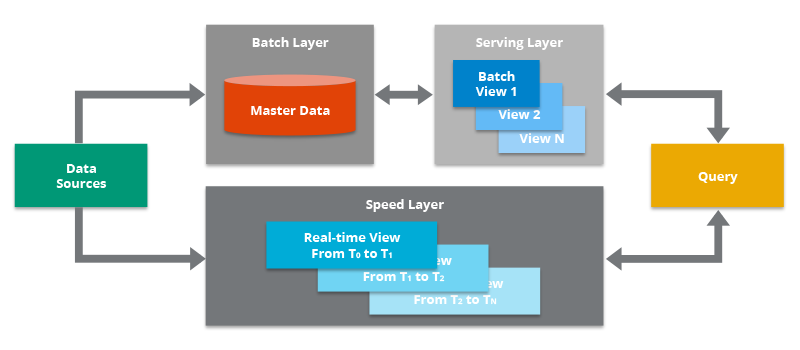
\includegraphics[width=\textwidth-10pt]{book-text/spark-architecture.png}
\end{figure}


In the case of user-similarity, let's work on a batch job implementation of computing a daily table; so first we'll need to get ratings from our schema before today, we also include a few other filters that simulate how this query might look in real life:

\begin{lstlisting}[language=Python]
user_item_ratings_qry = """
SELECT 
  book_ratings.book_id
  book_ratings.user_id
  , book_ratings.rating_value
  , book_ratings.rating_tstamp

FROM prod.book_ratings
JOIN prod.dim_users 
	ON book_ratings.user_id = dim_users.user_id 
JOIN prod.dim_books
	ON book_ratings.book_id = dim_books.dim_books

WHERE 
	DATE book_ratings.rating_tstamp 
		BETWEEN (DATE '2017-01-01') AND (CAST(current_timestamp() as DATE)
  AND book_ratings.rating_value IS NOT NULL
	AND dim_users.country_code = 'US'
  AND dim_books.book_active 
"""

user_item_ratings_sdf = spark.sql(user_item_ratings_qry)
\end{lstlisting}

As before, utilizing the SQL syntax to get the dataset into a Spark DataFrame is the first step, but now we have some additional work on the PySpark side. This is usually the pattern: get the dataset you want to work with via simple SQL syntax and logic, then use PySpark API to do some more detailed data processing.

Let's first observe that we have no assumptions about uniqueness in the above. For the sake of this table, let's decide that we'll use the most recent rating for a pair.

\begin{lstlisting}[language=Python]
from pyspark.sql.window import Window

windows = Window().partitionBy(
	['book_id', 'user_id']
).orderBy(
	col("rating_tstamp").desc()
)

user_item_ratings_sdf.withColumn(
	"current_rating", 
	first(
		user_item_ratings_sdf("rating_tstamp")
	).over(windows).as("max_rating_tstamp")
).filter("rating_tstamp = max_rating_tstamp")
\end{lstlisting}

We'll now use \lstinline{current_rating} as our ratings column for the purpose of downstream calculation.

Recall from before our ratings-based definition of user-similarity: 

\begin{equation}
\mathrm{USim}_{A,B}=\frac{\sum_{x\in \mathcal{R}_{A,B}}(r_{A,x}-\bar{r}_A)(r_{B,x}-\bar{r}_B)}{\sqrt{\sum_{x\in \mathcal{R}_{A,B}}(r_{A,x}-\bar{r}_A)^2} \sqrt{\sum_{x\in \mathcal{R}_{A,B}}(r_{B,x}-\bar{r}_B)^2}}    
\end{equation}



The important values we'll need are:

\begin{itemize}
\item $r_{(-,-)}$
\item $\bar{r}_{(-)}$
\end{itemize}

The rows are already the $r_{(-,-)}$ values, so let's compute user average ratings, $\bar{r}_{(-)}$ and the rating deviations:

\begin{lstlisting}[language=Python]
from pyspark.sql.window import Window
from pyspark.sql import functions as F

user_partition = Window.partitionBy('user_id')

user_item_ratings_sdf = user_item_ratings_sdf.withColumn(
	"user_average_rating", 
	F.avg("current_rating").over(user_partition)
)

user_item_ratings_sdf = user_item_ratings_sdf.withColumn(
	"rating_deviation_from_user_mean", 
	F.col("current_rating") - F.col("user_average_rating")
)
\end{lstlisting}

Now our schema should look like this (formatted slightly nicer than the default spark output):

\begin{lstlisting}[language=Python]
+-------+-------+------------+-------------+
|book_id|user_id|rating_value|rating_tstamp|
+-------+-------+------------+-------------+
+-------------+-------------------+-------------------------------+
current_rating|user_average_rating|rating_deviation_from_user_mean|
+-------------+-------------------+-------------------------------+
\end{lstlisting}

Let's finish creating a dataset that contains our User Similarity calculations:

\begin{lstlisting}[language=Python]
user_pair_item_rating_deviations = user_item_ratings_sdf.alias("left_ratings").join(
	user_item_ratings_sdf.alias("right_ratings"), 
  (
		F.col("left_ratings.book_id") == F.col("right_ratings.book_id") &\
		F.col("left_ratings.user_id") != F.col("right_ratings.user_id")
	),
	"inner"
).select(
	F.col("left_ratings.book_id"),
	F.col("left_ratings.user_id").alias("user_id_1"), 
	F.col("right_ratings.user_id").alias("user_id_2"),
  F.col("left_ratings.rating_deviation_from_user_mean").alias("dev_1"),
  F.col("right_ratings.rating_deviation_from_user_mean").alias("dev_2")
).withColumn(
	'dev_product', 
	F.col("dev_1")*F.col("dev_2")
)

user_similarities_sdf = user_pair_item_rating_deviations.groupBy(
	"user_id_1", "user_id_2"
).agg(
	sum('dev_product').alias("dev_product_sum"),
	sum(F.pow(F.col("dev_1"),2)).alias("sum_of_sqrd_devs_1"),
	sum(F.pow(F.col("dev_2"),2)).alias("sum_of_sqrd_devs_2")
).withColumn(
	"user_similarity",
	(
		F.col("dev_product_sum") / (
			F.sqrt(F.col("sum_of_sqrd_devs_2")) * F.sqrt(F.col("sum_of_sqrd_devs_2"))
		)
	)
)
\end{lstlisting}

We begin by taking a self join which avoids matching the same users with themselves, but joins on books that match. As we do this join, we take the rating deviation from user's mean ratings that we computed above. We also use this opportunity to multiply them together for the numerator in our user similarity function. In the last step, we'll groupBy again so that we can sum over all matching book ids (by groupBy on \lstinline{user_id_1} and \lstinline{user_id_2}); we sum the product and the powers of each set of deviations, so that we can finally divide and generate a new column for our user similarity. 

While this computation isn't particularly interesting, let's take note of a few things that we might appreciate. First, we built our user-similarity matrix in full from our records. This is something that may now be stored in a faster access format so that if we wish to do operations in real-time, it's ready to go. Second, we did all of the above in Spark, so we can run these operations on massive datasets and let spark handle the parallelization onto the cluster. We even were able to do this while writing code that looks a lot like pandas and sql. Finally, all the operations we did were columnar, and required no iteration-based calculation. This means this code will scale much better than some approaches. This also ensures that Spark can parallelize our code well, and we can expect good performance.

We've seen how PySpark can be used to prepare our user-similarity matrix. As an exercise, can you take this matrix and generate the Affinity matrix?

\begin{equation}
    \mathrm{Aff}_{A,i}=\bar{r}_A+\frac{\sum_{U\in \mathcal{N}(A)}\mathrm{USim}_{A,U}*(r_{U,i}-\bar{r}_A)}{\sum_{U\in \mathcal{N}(A)}\mathrm{USim}_{A,U}}
\end{equation}

Feel free to assume that $\mathcal{N}(A)$ is just the 5 nearest neighbors to $A$ with respect to user-similarity.

\subsection{Dataloaders}

As we begin to integrate gradient-based learning into our recommendation system architectures, we will face challenges in our MLOps tooling. The first of which is related to training data size and available memory. 

First let's recall the basics of \emph{Mini-Batched Gradient Descent}; during training via gradient descent, we make a forward pass of our training sample through our model to yield a prediction, we then compute the error and the appropriate gradient backwards through our model to update parameters. Batched Gradient Descent takes all of our data in a single pass to compute the gradient for the training set and push it back through–this implies you have the entire training dataset in memory. To avoid this, we can instead only compute gradients of the loss function for a subset of the dataset at a time. The simplest paradigm for this is called \emph{Stochastic Gradient Descent} and computes these gradients and parameter updates one sample at a time. The mini-batched version performs our batched gradient descent, but over a series of subsets to form a partition of our dataset. In familiar notation:

\begin{equation}
    \theta = \theta - \eta*\nabla_{\theta}J\left(\theta; x^{(i:i+n)};y^{(i:i+n)}\right)    
\end{equation}


This optimization serves a few purposes: first, it only requires potentially small subsets of our data in memory during the steps; second, it requires far less passes than the purely iterative version in SGD: third, the gradient operating on these mini-batches can be organized as a jacobian and thus we have linear-algebraic operations which may be highly optimized.

If you're convinced mini-batches are useful, then it's time to discuss \emph{Dataloaders}; a simple pytorch API for making mini-batch access from a large dataset much easier. The key parameters for a dataloader are \lstinline{batch_size}, \lstinline{shuffle}, and \lstinline{num_workers}. The batch size is easy to understand: it's the number of samples included in each batch (often an integer factor of the total size of the dataset). Shuffle allows the order to be randomized that batches in each epoch are shown to the network; this is intended to improve robustness. Finally \lstinline{num_workers} is a parallelization parameter for the CPU's batch generation.

The utility of a DataLoader is really best understood via demonstration:

\begin{lstlisting}[language=Python]
params = {
	'batch_size': _,
  'shuffle': _,
  'num_workers': _
}

training_generator = torch.utils.data.DataLoader(training_set, \emph{params)

validation_generator = torch.utils.data.DataLoader(validation_set, \emph{params)

\section{Loop over epochs}
for epoch in range(max_epochs):
    # Training
    for local_batch, local_labels in training_generator:

        # Model computations
        [...]

    # Validation
    with torch.set_grad_enabled(False):
        for local_batch, local_labels in validation_generator:

            # Model computations
            [...]
            \end{lstlisting}

The first important detail in the above is that any the generators above will be reading in minibatches from your total dataset, and can be instructed to load those batches in parallel. Note also that any differential steps in the model computations will now be operating on these minibatches. 

It's easy to think of Dataloaders as merely a tool for code cleanliness–which admittedly it does improve–but it's important to not underestimate how the control of batch order, parallelization, and shape are significant features for training your model. Lastly, the structure of your code now looks like Batch Gradient Descent, but is taking advantage of mini-batching, further exposing what your code actually does instead of the steps necessary to do it.

\subsection{Database snapshots}

Let's round out this section by stepping back from these fancy technologies, to discuss something important and classic–snapshotting a production database.

An extremely likely scenario, is that the engineers(potentially also you) who have built the application your recommendations will be served via, are writing their logs and other application data to a SQL database. More likely than not, this database architecture and deployment are optimized for fast querying by the application across the application's most common use-cases. As discussed above, those logs may be in an event-style schema, and there may be other tables that require aggregation and rollup to make any sense–for example a 'current inventory' table may require knowledge of start-of-day inventory and then aggregate a list of purchase events.

All told, the production SQL database is usually a crucial component in the stack, that's geared at specific use. As the downstream consumer of this data, you may find yourself wanting different schema, wanting lots of access to this database, and performing serious operations on these data. The most common paradigm is \emph{database snapshotting}. Snapshotting is a functionality provided by various flavors of SQL to performantly make a clone of a database. While there are a variety of ways this shapshotting may take form, let's focus on a few ways to use these shapshots to serve our purposes.

\begin{itemize}
\item A daily table snapshot may be tied to an \lstinline{as_of} field, or \emph{the state of this table on this day}
\item A daily table snapshot may be limited by time to see \emph{what records have been added today}
\item An event table snapshot may be used to feed a set of events into some event stream processor like Segment (note that you may also set up live event streams like Kafka)
\item A hourly aggregated table can be used for status logging or monitoring
\end{itemize}

In general, the paradigm is usually to operate on snapshots for downstream data processing. Many of the kinds of data processing we mentioned earlier–like computing user similarity–are operations that may require significant data reads. \emph{It's important to not build ML applications that require extensive querying on the production database,} it will likely decrease performance of the app and result in a slower user experience. This decrease will undermine the improvement made possible by your recommendations. 

Once you've snapshotted the tables you're interested in, there's often a collection of data pipelines useful to transform those data into even more specific tables in your \emph{data warehouse}–where you should be doing most of your work anyhow. Tools like Airflow, Argo, and Luigi are popular data pipeline and workflow orchestration tools for ETL. 

\section{Data Structures for learning and inference}

\begin{enumerate}
    \item Vector search/ANN index
    \item Bloom filters for candidate filtering
    \item Feature stores
\end{enumerate}

Previously we discussed the necessary components for getting data flowing in your system. Now we'll see some strategies for how you organize data to make it more accessible during the learning and inference processes. Also we'll find some shortcuts to speed things up during retrieval. 

\subsection{Vector search}

We have learned about user-similarity and item-similarity for understanding the relationships between those entities accordingly, but we haven't talked about any \emph{acceleration structures} for these processes. 

First let's discuss a bit of terminology; if we think of a collection of vectors that represent entities with a similarity metric provided by a distance function, we refer to this as a \emph{latent space.} The simple goal is to utilize our latent space and it's associated similarity metric (or complimentary distance metric) to be able to retrieve \emph{similar} things quickly. In our previous examples with similarity we talked about neighborhoods of users, and how they can be utilized to build an affinity score between users and unseen items. But how do you find the neighborhood?

First, recall that we defined neighborhoods of an element $x$, written $\mathcal{N}(x)$, as the set of $k$-elements in the latent space with the maximum similarity; or said differently the set of $j$'th order statistics for $j\leq k$ from the sample of item similarities to $x$. These \emph{$k$-nearest neighbors}, as they're often referred, will be used as the set of elements considered similar to $x$.

In addition, to using these vectors for the purely collaborative-filtering definitions before we can use them in other ways. 

\begin{itemize}
\item a simple recommender that randomly samples unseen items from a user neighborhood's liked items
\item predicting features of a user from known features of users in the neighborhood
\item user segmentation via taste-similarity
\end{itemize}

So how can we speed up these processes? One of the first significant improvements in this area came from what are called inverted-indices; which at it's core is carefully constructing a large hash between tokens of the query(for text based search) and the candidates. 

This approach is great for tokenizable entities like sentences, or small-lexicon collections. Given the ability to look up items which share one or many tokens with the query, you can even use a general latent embedding to rank the candidate-responses by similarity. Unfortunately, this does incur a speed cost as it is two steps, and because the similarity distribution may not be well correlated with the token similarity we'd need to return many more candidates than we need.  

In fact, one can do better. Instead of only building these indices for tokenizable components of your elements, you could pre-compute the \emph{KD-tree} and use those as the index. KD-trees are an efficient data-structure for encoding the above neighborhoods, but are notoriously slow to read from in higher dimensions. Using them instead to build inverted indices though can be a great improvement. 

More recently, explicitly using vector-databases with vector search is becoming much more possible and feasible. Elasticsearch has added this capability, FAISS and Pinecone are a vector-database system explicitly targeting this goal, and Weaviate is a native vector-database architecture that allows you to layer the previous token-based inverted indices and vector similarity search.

\paragraph{Approximate Nearest Neighbors}

It turns out that you often are satisfied with approximate solutions to the question: what are this element's k-nearest neighbors. Incredibly, the field of approximate nearest neighbors can get very high accuracy compared to the actual nearest neighbors, and with head-spinning speedups.

One such library is [PyNNDescent]\url{https://github.com/lmcinnes/pynndescent}) which uses clever speedups via both optimized implementation and careful mathematical tricks. With ANN, you are opened up to two different strategies from above:

\begin{itemize}
\item pre-index can be dramatically improved
\item on queries without a pre-indexing option, you can still expect good performance.
\end{itemize}

In practice, these similarity lookups are incredibly important for making your applications actually work. While we've mostly talked thus far about recommendations for full known catalogs of items, there are other recommendation contexts where we cannot assume this:

\begin{itemize}
\item query-based recommendations (like search)
\item contextual recommendations
\item cold-starting new items
\end{itemize}

As we go we will see more and more references to similarity in spaces and nearest neighbors; at each of those moments think: 'I know how to make this fast!"

\subsection{Bloom filters}

Via vector search we have identified a large pool of potential recommendations for the user. From this pool, we need to do some immediate elimination. The most obvious type of high-level filtering that's essential is to remove those items that the \emph{user has previously not shown interest in, or has already purchased.} You've probably had the experience of being recommended the same item, over and over, and thinking "I don't want this, stop showing me this". From the simple collaborative filtering models we've introduced, you may now see why this could happen. 

The system has identified a set of items via collaborative filtering that you're more likely to pick. Without any outside influence, those computations will continue to return the same results, and thus you'll never escape those recs. As the system designer, you may start with a heuristic:

\vspace{10pt}
\colorbox{almond}{\parbox{\textwidth}{
If the user has seen this item recommended 3 times, and never clicked, let's not show it to them anymore.
}}
\vspace{10pt}

This is a totally reasonable strategy to improve what is often called "\emph{freshness}" in your recommendation system. While this is a simple strategy to improve your recommendations, how might you actually implement this at scale? 

Bloom filters are probabilistic data structures, that allow one to test for set inclusion very efficiently, with a downside: set exclusion is deterministic, but set inclusion is probabilistic. \emph{In practice this means that asking the question "is $x$ in this set" never results in a false negative, but may result in a false positive!} Note that this type-I error increases as the size of the bloom increases. 

A bloom filter may be used in our above freshness strategy by using defining the set's in question to be: "has this user seen this item recommended 3 times and never clicked". Bloom filters have a caveat that they're additive-only, i.e. once somethings in the bloom, you can't remove it. This is not a problem when observing a binary state like this heuristic.

Let's construct a user-item id to use as our hash in the bloom, remember that the key feature of the bloom filter is to very quickly determine if the hashed item is in the bloom. When we observe a user-item pair that satisfies the criteria above, take that pair as an id and hash it. Now, because that hashed pair is easily reconstructable from a list of items for a user, we have a very fast way to filter.

Let's discuss a few technical details on this topic. There may actually be a variety of kinds of filtering you wish to do–maybe freshness is one, and another may be items they already own, and a third that says to exclude items that have sold out.

Here it would be good to implement each of these filters independently; the first two can follow our user-item id hashing as before, and the third one can be a hash only on item ids.

Another consideration is populating the bloom filters. It's best practice to build these blooms from a database during the offline batch jobs. On whatever schedule your batch training is run, rebuild your blooms from the records storage to ensure you're keeping your blooms accurate. Remember that blooms don't allow deletion, so in the previous example if an item goes from sold-out to re-stocked, your batch refresh of your blooms can pick up the availability again. In between batch retraining, adding to a bloom is also very performant, so you can continue to add to the bloom as you observe more data that needs to be considered for the filtering in real-time. Be sure these transactions are logged to a table though! It'll be important when you want to refresh. 

\paragraph{Fun aside: bloom filters \emph{as} the recommendation system}

In addition to bloom filters creating an effective way to eliminate some recommendations based on conditions for inclusion, there's a creative–and effective–application of bloom filters to doing the recommending itself! In particular, it was shown in \url{https://hal.archives-ouvertes.fr/hal-01314910/document} that for high dimensional feature sets, with a lot of sparsity(as we discussed in the introduction), the type of hashing bloom filters do, can help overcome some of the key challenges in defining good similarity functions!

Let's observe that there are two natural operations that one can do on sets, via the bloom filter data structures. First, consider two sets $A$ and $B$, and associate to them bloom filters $\mathcal{BF}_A$ and $\mathcal{BF}_B$, then what's the definition of $A\cap B$? Can we come up with a bloom filter for this intersection? Yep! Recall that our bloom filters are guaranteed to tell us when an element is not contained in the set, but only probabilistic for when it is. In this case, we'd simply look for elements that are 'in' according to $\mathcal{BF}_A$ \emph{AND} 'in' according to $\mathcal{BF}_B$. Of course, the set of items returned as 'in' each set is larger than the actual set, i.e. $A\subset \mathcal{BF}_A$, so the intersection will also be larger:

\begin{equation}
    A\cap B \subset \mathcal{BF}_A \cap \mathcal{BF}_B.
\end{equation}

Note that you can compute exactly the difference in cardinality via information about your choice of hashing functions. Also note that the above is an abuse of notation by calling $\mathcal{BF}_A$ the set of things returned by the bloom filter corresponding to $A$.

Second, we need to construct also the union. This is similarly easy by considering elements that are 'in' according to $\mathcal{BF}_A$ \emph{OR} 'in' according to $\mathcal{BF}_B$. And so, similarly:

\begin{equation}
    A\cup B \subset \mathcal{BF}_A \cup \mathcal{BF}_B.
\end{equation}

Now, if we consider items $X$ and $Y$ as concatenated vectors of potentially many features, and hash those concatenated features, we are representing each of them as the bitwise vectors of our bloom. From before, we saw that the intersection of two blooms makes sense, and in fact is equivalent to the bitwise \emph{AND} of their bloom representations. This means two items' feature similarities, can be expressed by the bitwise AND similarity of their bloom hashes:

\begin{equation}
    \mathrm{sim}(X,Y)=|\mathcal{BF}(X)\cap \mathcal{BF}(Y)|=\mathcal{BF}(X)\cdot_{\mathrm{bitwise}}\mathcal{BF}(X)
\end{equation}

For datasets that are static, this method has some real advantages including speed, scalability, and performance. There are limitations based on variety of features, and the ability to change the set of possible items. Later we will discuss \emph{Locally Sensitive Hashing} and some similar ideas will re-emerge. 

\subsection{Feature stores}

So far, we have focused on recommendation systems that one might call "pure collaborative filtering". That is to say that we've only made use of the user or item similarity data when attempting to make good recommendations. If you've been wondering "hey, what about information about the actual users and items?"; your curiosity will now be sated. 

There are a huge variety of reasons why you could be interested in features in addition to your collaborative filtering methods of before. Let's list a few high level concerns:

\begin{itemize}
\item you may wish to show new users a specific set of items first
\item you may wish to consider geographic boundaries in your recommendations
\item it may be important to distinguish between children and adults for the types of recommendations they're given
\item item features may be used to ensure high-level diversity in the recommendations (more to come on this later)
\item user features can enable various kinds of experimental testing
\item item features could be used to group items into sets for contextual recommendations (more to come on this later)
\end{itemize}

In addition to the above, there's a separate kind of features that are often essential: real-time features. While the point of feature stores is to provide real-time access to all the necessary features, it's worthwhile to distinguish the stable features which change infrequently from the real-time features which we anticipate changing very often. 

Some important examples of a real-time feature store are dynamic prices, current item availability, 'trending' status, wishlist status, and so on. These features may change throughout the day, and we want their values in the feature store to be mutable in real-time via other services and systems. This means that the real-time feature store will need to provide API access for feature mutation. This is something you may not want to provide for the 'stable' features.

When we design our feature store, we're likely to want the 'stable' features to be built from Data Warehouse tables via some ETLs and transformations, and the real-time feature store to be also, but on a faster schedule, or allow API access for mutation. In either case, the key quality of a feature store is \emph{very fast read access}. It's often a good idea to separately build feature stores for offline training of models that can be built in test to ensure support for new models.

So how might the architecture and implementation look?

\begin{figure}[h!]
    \caption{https://www.tecton.ai/blog/what-is-a-feature-store/}
    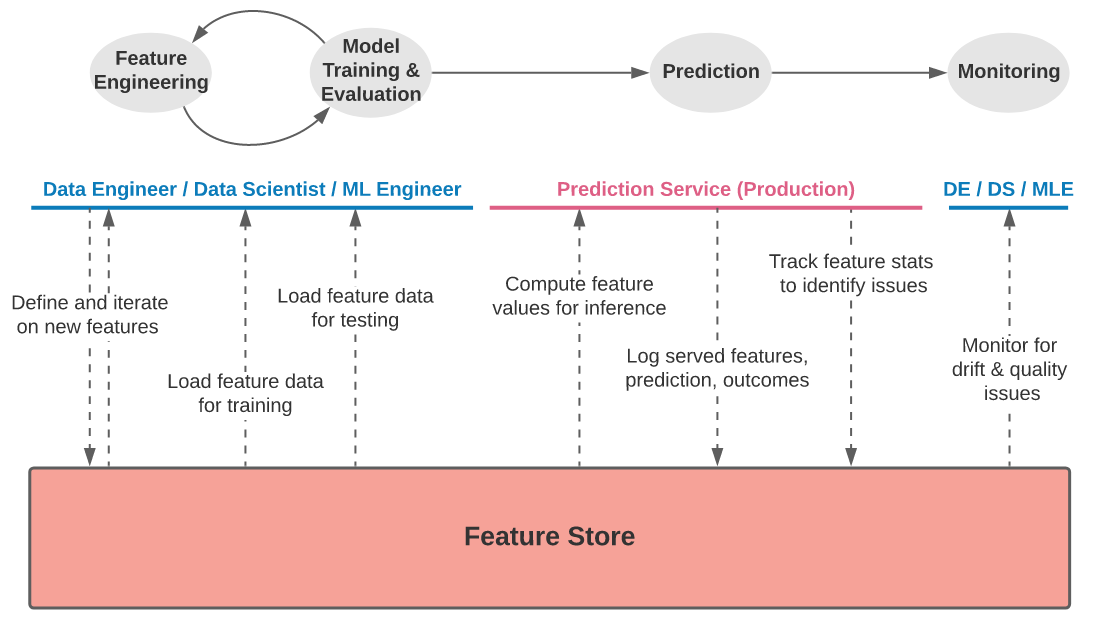
\includegraphics[width=\textwidth-10pt]{book-text/feature-store.png}
\end{figure}

Designing a feature store involves designing pipelines that define and \emph{transform the features into that store}–coordinated via things like Airflow, Luigi, Argo, etc.–and often look similar to the type of data pipelines used in building our collector. One additional complication that the feature store needs to concern itself with is a speed layer. We mentioned before that for the collector, we can think of batch data processing and a more rapid speed layer for intermediary updates, but for the feature store this is even more important. The feature store may also need a \emph{streaming layer}. The streaming layer is something that operates on continuous streams of data, and can perform data transformations on those; it then writes the appropriate output to the online feature store in real time. The reason this adds complexity is because data transformations on streaming data are a very different set of challenges, and often require different algorithmic strategies. Some technologies that help here are Spark Streaming or Kinesis. You'll also need to configure system to properly handle the data stream; the most common of which is Kafka.

A feature store also needs a \emph{storage layer}; a large variety of different approaches exist here, but it's very common to use a NoSql database especially in the online feature store. This is because of faster retrieval and the nature of the data storage. Feature stores for recommendation systems tend to be very key-based, i.e. 'get the features for this user', or 'get the features for this item', which lend themselves well to key-value stores. Some example technologies here are DynamoDB, Redis, and Cassandra. The storage layer for offline feature store may simply be a Sql style database to reduce complexity, but instead you'll pay a tax of a delta between offline-and-online. This delta, and others like it are call [training-serving skew]\url{https://developers.google.com/machine-learning/guides/rules-of-ml#:~:text=Training%2Dserving%20skew%20is%20a,train%20and%20when%20you%20serve.}).

A unique but essential aspect of feature stores is the \emph{registry}. A registry is incredibly useful for a feature store because it coordinates what features exist, and some information on how they're defined. A more sophisticated instance of a registry also includes input and output schemas with typing, and distributional expectations. These things are contracts that the data pipelines must adhere to and satisfy to avoid populating your feature store with garbage data. Additionally the registry's definitions allow parallel Data Scientists and ML Engineers to develop new features, use each others features, and generally understand the assumptions of features their models may utilize. One important advantage of these registry is that they incentivize alignment between teams and developers–in particular, if you decide you care about 'country' for your user, and you see that there is a feature 'country' in the registry, you're more likely to just use that (or ask the developer who's assigned to this feature in the registry) than make a new one from scratch. Practically, there are hundreds of small decisions and assumptions data scientists make when defining features for their models, this removes some of that load be relying on the existing resources.

Finally, we need to talk about \emph{serving} these features. Backed by the appropriately performant storage layer, we need to serve via API request the feature vectors necessary. The API can serve back the entire set of features for the key, or allow for more specification. Often the responses are JSON serialized for fast data transfer. It's important that the features be served are the \emph{most up to date set of features}, and latency here is expected to be <100ms for more serious industrial applications. One important caveat here is that for offline training, these feature stores need to accommodate \emph{time-travel}. Because our goal during training is to give the model the appropriate data to learn in the \emph{most generalizable way}, when training our model it's crucial to not give it access to features out of time. This is called \emph{data-leakage} and can cause massive divergence in performance between training and prod. The feature store for offline training thus must have knowledge of the features through time, so that during training, a time index may be provided to get the features as they were then. These \lstinline{as_of} keys can be tied to the historical training data as we 'replay' history of what the user-item interactions looked like.

With these pieces in place–and the important monitoring this system needs–you'll be able to serve offline and online features to your models. Later we will see model architectures that make use of them.

\paragraph{Data leakage}

Data leakage in machine learning is broken up into \emph{feature leakage} and \emph{training example leakage}. For recommendation systems, data leakage has the additional challenge of temporal leakage or non-stationarity leakage. The real danger is that in recommendation systems, we see the same observational unit, a user, over and over, and observe a datum each time we see them. When we see them, other aspects of the system may have changed, and in reality we want to use features in our model that are the most up-to-date as of that observation. Both in features and training examples, to avoid leakage we need to always be thinking of the timeline of our system. This is why data preparation for recommendation systems is inherently time-dependent. We will see later that our accuracy metrics will need to explicitly consider train-test splitting with respect to this time axis, and then further grouped by the user. This also means that training recommendation systems often requires more resources than many other task types.